\documentclass{article}[18pt]
\usepackage{../../../../format}
\lhead{Software Engineering - Project Management}


\begin{document}
\begin{center}
\underline{\huge Your Team, Skills and Starting Points}
\end{center}
\section{Skills}
\subsection{Skills Audit}
A clear understanding of not only your role but what are the strengths and weaknesses of your skill set is vital
\begin{center}
	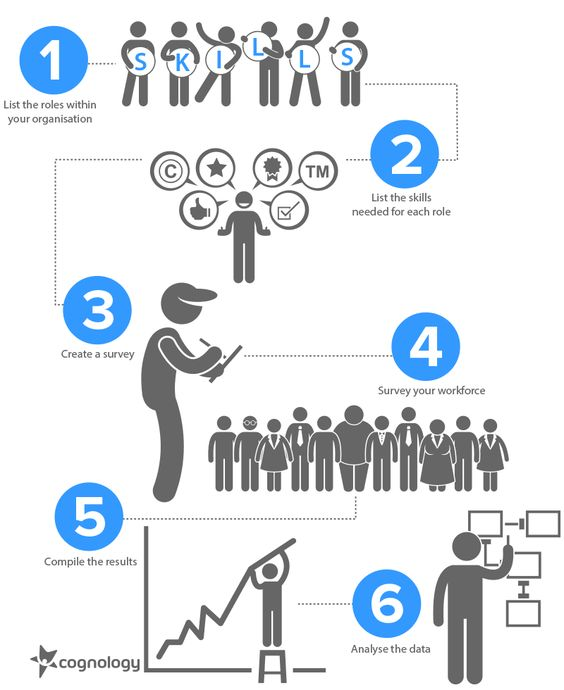
\includegraphics[scale=0.7]{Audit}
\end{center}
\subsection{Four Stages of Competence}
\textbf{Unconscious Incompetence} - You are unaware of the skills and your lack of proficiency\\
\textbf{Conscious Incompetence} - You are aware of the skill but not yet proficient\\
\textbf{Conscious Competence} - You are able to use the skill, but only with effort\\
\textbf{Unconscious Competence} - Performing the skill becomes automatic
\subsection{Dunning Kruger Effect}
\begin{center}
	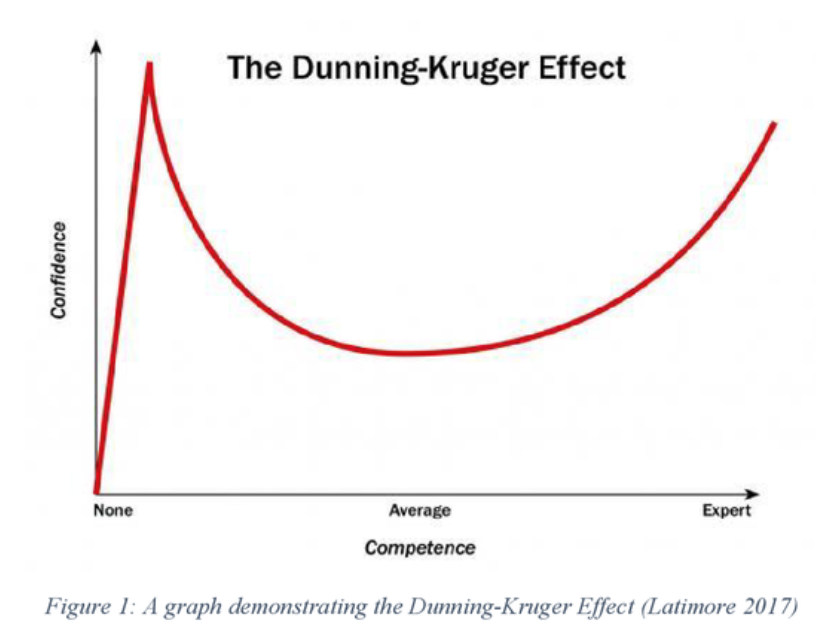
\includegraphics[scale=0.7]{Dunning_Kruger}
\end{center}
\subsection{Skill Development Plan}
\begin{itemize}
	\item Create a team based CPD plan
	\item Assign parts of the plan to individuals
\end{itemize}
\subsection{CPD Plan}
\begin{center}
	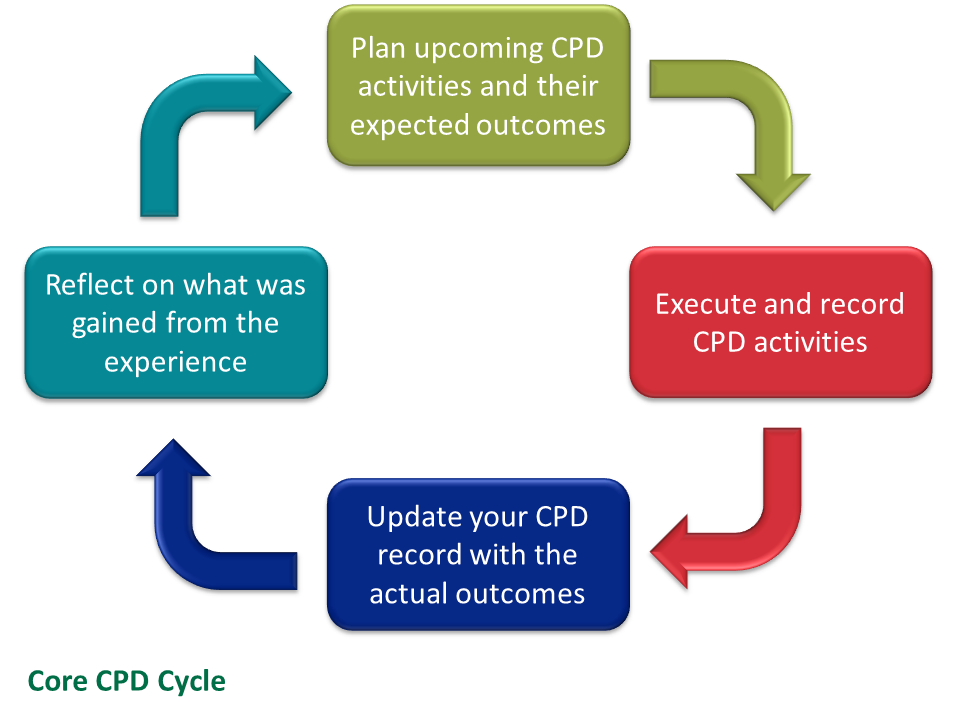
\includegraphics[scale=0.7]{Plan}
\end{center}
\section{Ideation}
\begin{center}
	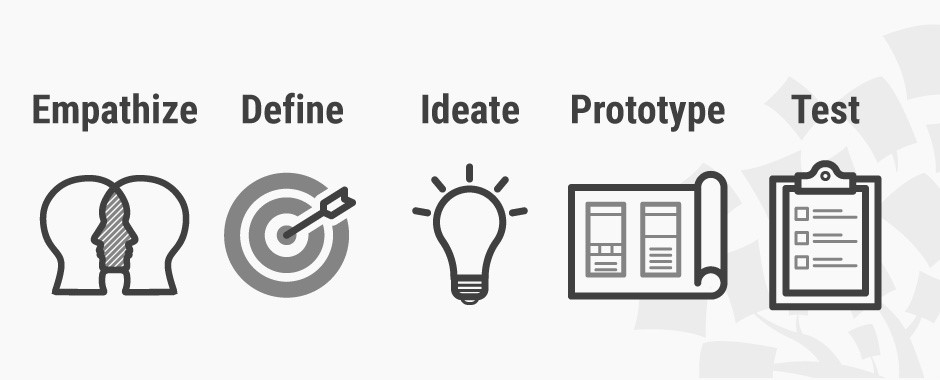
\includegraphics[scale=0.7]{Ideation}
\end{center}
Empathise:
\begin{itemize}
	\item Gain an understanding of the problem, normally through user research
	\item Crucial to a human centred design process (P.A.C.T.)
\end{itemize}
Define:
\begin{itemize}
	\item Analyze your observations and synthesize them to define the core problems
	\item Define sub-problems
\end{itemize}
Ideate:
\begin{itemize}
	\item Generate ideas
	\item Lateral thinking stage
	\item Often the innovation stage, especially if you can put your own assumptions and prejudices behind you
\end{itemize}
Ideation Approaches:
\begin{itemize}
	\item \textbf{Brainstorming} - You build good ideas from each other's wild ideas
	\item \textbf{Braindumping} - This is like brainstorming, but don individually
	\item \textbf{Brainwriting} - This is like brainstorming, but everyone writes down and passes ideas for other others to add to before discussing these
	\item \textbf{Worst Possible Idea} - You take an inverted brainstorming approach, emboldening more reserved individuals to produce bad ideas and yielding valuable threads
	\item \textbf{Challenging Assumptions} - You overturn established beliefs about problems, revealing fresh perspectives
	\item \textbf{Mindmapping} - You use this graphical technique to connect ideas to problems' major and minor qualities
	\item \textbf{Bodystorming} - You use role-playing in scenarios/customer-journey steps to find solutions
	\item \textbf{Provocation} - You use an extreme lateral-thinking technique to challenge established beliefs and explore paths beyond
\end{itemize}





\end{document}